\documentclass[11pt,a4paper]{article}

\usepackage[a4paper,margin=2.4cm]{geometry}
\usepackage{graphicx}
\usepackage{booktabs}
\usepackage{caption}
\usepackage{subcaption}
\usepackage{amsmath,amssymb}
\usepackage{microtype}
\usepackage{xcolor}
\usepackage[hidelinks]{hyperref}
\usepackage{enumitem}
\usepackage{titlesec}
\usepackage{titling}
\usepackage{placeins}
\usepackage{float}

\definecolor{accent}{HTML}{2E6FB3}
\definecolor{benefit}{HTML}{1F7A5A}
\definecolor{harm}{HTML}{C0392B}

\titleformat{\section}{\Large\bfseries\color{accent}}{\thesection}{0.6em}{}
\titleformat{\subsection}{\large\bfseries}{\thesubsection}{0.5em}{}

\setlength{\parskip}{0.45em}
\setlength{\parindent}{0pt}
\captionsetup{font=small,labelfont=bf,margin=8pt}

\setlength{\droptitle}{-2.5em}
\title{\bfseries A guarded causal-inference pipeline for EHR-derived treatment-policy questions:\\
\large operationalising causal guardrails, with a worked example in ICU antibiotic continuation}
\author{Lukas Schmidt\\
\small Technical University of Munich, inContAlert}
\date{\today}

\begin{document}
\maketitle
\vspace{-1.5em}

%─────────────────────────────────────────────────────────────────────────────
\begin{abstract}
\small
Observational causal-effect estimates from electronic health records routinely overstate evidence: identification assumptions are not testable, diagnostics are scattered across packages, and modelling choices accumulate silently. We present a guarded causal-inference pipeline whose contribution is a \emph{refusal-to-render contract}: every effect estimate is paired, by construction, with the diagnostic that adjudicates it, and any contrast whose probe fails is suppressed from the rendered output. The components are familiar (target-trial emulation, doubly-robust estimation, multinomial generalized propensity scores, overlap and balance diagnostics, E-values, label-shuffle stability checks, simulation-based coverage); the contribution is the gating contract and its operational discipline. We illustrate the framework on a three-arm target trial of broad-spectrum antibiotic continuation in 9{,}314 sepsis-3 ICU stays from MIMIC-IV, with external validation on eICU-CRD. Two of the three pairwise contrasts are refused: the overlap probe fails on continue-vs-de-escalate (36\,\% in common support) and the deployment-layer calibration probe fails on the de-escalate arm (slope $0.34$). On the third contrast, cease-vs-continue 28-day mortality, the framework returns a fragile verdict via three independent diagnostics: (i) eight benchmark estimators disagree by $\sim$10\,pp (matched ATT $+1.5$\,pp [$-2.3$, $+3.9$], doubly-robust cluster at $-3.6$ to $-4.3$\,pp, stabilised IPTW $-8.5$\,pp), (ii) only $33\,\%$ of confounders satisfy $|$SMD$|<0.1$ after weighting, and (iii) the E-value is $1.55$ at the point estimate and $1.30$ at the CI bound nearest the null. Simulation-based coverage on a calibrated parametric mimic of the cohort spans $10\,\%$ (g-computation, under-covering) to $100\,\%$ (TMLE, over-wide), confirming that no single estimator is uniformly trustworthy in this setting. The doubly-robust cluster around $-4$\,pp is therefore retained as the framework's worked output, not as a stewardship recommendation. The pipeline, the pre-specification, and the diagnostic-gated reference frontend are released as a single reproducible artefact.
\end{abstract}

%─────────────────────────────────────────────────────────────────────────────
\section*{Author summary}

Causal-effect estimates from electronic health records are easy to compute and hard to defend: identification assumptions are not testable, model and feature choices propagate quietly, and diagnostics are often run as one-off scripts after the fact. We describe a pipeline whose contribution is the discipline of \emph{refusing to render}: every effect estimate produced is paired, by construction, with the diagnostic that adjudicates it, and any contrast whose probe fails is suppressed from the rendered output. The ingredients of the pipeline are familiar --- a target-trial protocol, doubly-robust estimation, a multinomial generalized propensity score, overlap and balance diagnostics, E-values, simulation-based coverage --- but the refusal contract is what we argue is missing from most applied observational causal-ML studies and what we are advocating as a structural change to how such studies are reported. We instantiate the framework on a three-arm target trial of broad-spectrum antibiotic continuation in ICU sepsis (MIMIC-IV, with external validation on eICU-CRD). The framework refuses to render two of the three pairwise contrasts: continue-vs-de-escalate fails the overlap probe and de-escalate-vs-stop fails the per-arm calibration probe. On the third contrast, cease-vs-continue, the framework returns a \emph{fragile} verdict --- eight benchmark estimators disagree by roughly 10 percentage points on the same cohort under the same generalized propensity score, two-thirds of the confounders fail post-weighting balance, and the E-value indicates a clinically plausible unmeasured confounder could fully explain the doubly-robust cluster of point estimates. The worked example is illustrative, not confirmatory: the framework's job in this paper is to expose the fragility, not to argue that one arm is safer than another.

%─────────────────────────────────────────────────────────────────────────────
\section{Introduction --- operationalising causal guardrails in EHR studies}

Causal-inference methods for observational EHR data are now standard equipment: target-trial emulation \cite{hernan2016target}, doubly-robust estimation including double/debiased machine learning (DML) \cite{chernozhukov2018dml}, propensity overlap, E-values \cite{vanderweele2017evalue}, calibration assessment, and label-shuffle placebos. Each is well documented in isolation. In practice, however, they are seldom assembled into a single workflow, and the most common failure mode of an applied causal-ML paper is not the absence of any one diagnostic but the diffuse, unauditable way the diagnostics are bolted on after the fact. The reader sees an effect estimate; the diagnostic that would tell them whether to trust it lives in a different table, a different notebook, or no longer exists. Integrative templates exist (Doutreligne et al.\ 2024 \cite{doutreligne2024stepbystep}; the broader target-trial-emulation literature) but they describe \emph{what} an analyst should do; they do not bind the rendering of an effect estimate to the verdict of its diagnostic.

This paper does not introduce a new estimator. It describes a pipeline whose contribution is a \emph{refusal-to-render contract}: a formal binding between probes and rendered outputs such that an effect estimate cannot be displayed unless its supporting diagnostic has been computed and has not failed. We define the contract in \S\ref{sec:contract} as a small set of probe-to-render rules, and we argue --- and demonstrate, in the worked example --- that this discipline is the single cheapest improvement available to applied observational causal-ML before any new methodological work. The components of the pipeline are familiar (target-trial protocol; DML and a benchmark grid that includes DRLearner, AIPW, stabilised IPTW, overlap-weighted IPTW \cite{li2018overlap}, TMLE \cite{vanderlaan2011tmle}, $g$-computation, and propensity matching; multinomial generalized propensity score; E-values; balance and overlap diagnostics; simulation-based coverage; specification-stability checks); the contract is what binds them.

We instantiate the pipeline on a representative observational decision: continuation versus de-escalation versus cessation of broad-spectrum antibiotics at 72\,h in ICU sepsis. We choose this case because (i) it is the canonical confounding-by-indication problem --- clinician-intent variables (frailty gestalt, code status, undocumented improvement, ID-consult input) are partially or fully unobserved in any retrospective EHR study and the pipeline must therefore be able to estimate \emph{and} to publicly fail; (ii) the downstream consequences of a guard mis-firing are clinically high-stakes (antimicrobial stewardship and patient mortality), so the cost of a false-confidence estimate is concrete; and (iii) the question admits external validation on a second large database. The framework refused two of the three pairwise contrasts in MIMIC-IV and returned a fragile-verdict on the third. We present the resulting numbers as the framework's worked output, not as a stewardship recommendation. The framework itself is intended to generalise to other treatment-policy questions in EHR data and to other databases: we exercise it across two databases (MIMIC-IV and eICU-CRD) and eight estimators.

\paragraph{Related work --- what is new.} Step-by-step causal-analysis templates for EHRs exist \cite{hernan2016target,doutreligne2024stepbystep}; benchmark suites compare estimators on synthetic and semi-synthetic data \cite{econml,vanderlaan2011tmle}; the E-value \cite{vanderweele2017evalue} and overlap-weighting \cite{li2018overlap} literatures provide individual sensitivity tools; reporting checklists (TRIPOD-AI, STROBE, RECORD-PE) prescribe documentation. What none of these provide --- and what this paper proposes --- is a binding contract between a probe and the rendered output: in the framework presented here, an effect estimate that lacks an evaluated probe, or whose probe fails, is structurally inaccessible in the released artefact (suppressed from the manuscript table, the CDSS display, and the JSON payload). The closest prior work is Doutreligne et al.\ 2024 \cite{doutreligne2024stepbystep}, which prescribes the steps but leaves the rendering decision to the analyst; we differ in making that decision a property of the pipeline rather than of the analyst's discipline.

%─────────────────────────────────────────────────────────────────────────────
\section{Framework}

\begin{figure}[H]
  \centering
  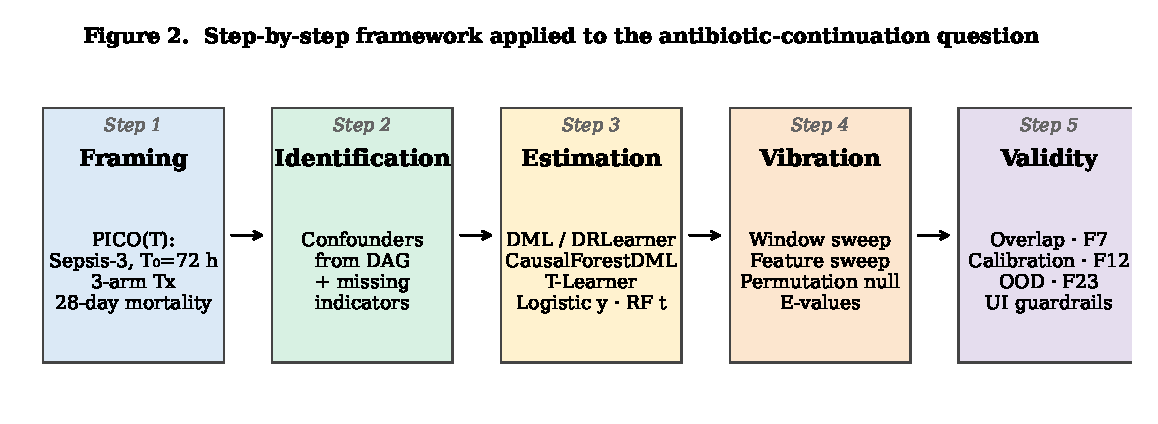
\includegraphics[width=\linewidth]{figures/fig2_framework.pdf}
  \caption{The five-step analytic pipeline used for the antibiotic-continuation question. Each step has its own audit artefacts and diagnostics; the design refuses to display an ATE for which the matching diagnostic is missing or has failed.}
  \label{fig:framework}
\end{figure}
\FloatBarrier

\subsection{The refusal-to-render contract}\label{sec:contract}

We formalise the gating discipline as a contract between probes and rendered outputs. For a target estimand $\theta$ (a pairwise ATE, ATT, or ATO on a chosen outcome), the pipeline evaluates a fixed set $\mathcal{P} = \{P_1, \dots, P_k\}$ of probes, each of which returns a verdict $v_i \in \{\text{pass}, \text{marginal}, \text{fail}\}$ together with a quantitative diagnostic value (e.g.\ \% of cohort in common support, $|$SMD$|<0.1$ fraction, E-value, simulation coverage). For each rendered surface $S \in \{\text{manuscript table}, \text{CDSS individual-risk display}, \text{JSON payload}\}$ the pipeline applies a render rule
\[
  R_S(\theta) \;=\; \begin{cases}
    \text{display}(\hat{\theta}, \text{CI}, \{(P_i, v_i)\}_i) & \text{if } \forall P_i \in \mathcal{P}_S^{\text{req}}: v_i \neq \text{fail} \\
    \text{suppress with reason}(\{P_i: v_i = \text{fail}\}) & \text{otherwise}
  \end{cases}
\]
where $\mathcal{P}_S^{\text{req}} \subseteq \mathcal{P}$ is the probe subset required for surface $S$. The set $\mathcal{P}$, the verdicts, and the rules are released alongside the manuscript in machine-readable form (\texttt{paper/preregistration.yaml} and the run-time \texttt{diagnostics\_summary.json}); the manuscript output table (Table~\ref{tab:summary}) is itself generated by $R_{\text{table}}$ rather than written by hand.

Three properties follow from this construction. (i)~\emph{Completeness}: the pipeline cannot render an effect estimate whose required probe is missing --- the rendering function depends on the probe's existence as a code-level pre-condition. (ii)~\emph{Auditability}: every failed render carries a probe-attributable reason, recorded in the JSON payload and surfaced in the table and CDSS. (iii)~\emph{Locality}: each surface $S$ has its own $\mathcal{P}_S^{\text{req}}$, so a probe that fails identification (overlap, E-value) suppresses an effect from the manuscript table, while a probe that fails individual-level reliability (per-arm calibration, Mahalanobis OOD) suppresses an arm from the CDSS without removing the population-level estimate from the methods table. The identification-layer vs.\ deployment-layer separation that we describe in Step 5 is the operational consequence of locality.

For the worked example, the required probe set is $\mathcal{P}^{\text{req}} = \{\text{overlap}, \text{post-weighting balance}, \text{E-value}, \text{specification-stability null}, \text{simulation coverage}\}$ for the manuscript table and additionally $\{\text{per-arm calibration}, \text{Mahalanobis OOD}\}$ for the CDSS. In MIMIC-IV the contract suppresses two of the three pairwise contrasts; in the third it renders the estimate accompanied by every probe's verdict (\S\ref{sec:summary}, Table~\ref{tab:summary}).

\subsection{Step 1 --- Target-trial protocol}
We frame the worked example as an emulation of a hypothetical randomised target trial. We follow the reviewer formulation in describing the contrast as an \emph{observed treatment-state comparison at $T_0$}, not as the effect of a deterministic treatment policy.

\begin{table}[H]
  \centering
  \small
  \caption{Target-trial protocol (left) and observational emulation (right). Each row is one Hernán--Robins protocol element. Items marked $^\dagger$ deviate from a strict target-trial emulation and are reported as sensitivity analyses.}
  \label{tab:protocol}
  \begin{tabular}{p{0.36\linewidth}p{0.56\linewidth}}
    \toprule
    Target trial & Observational emulation \\
    \midrule
    \emph{Eligibility} & Adult ICU sepsis-3 admissions, ICU LOS $\geq 72$\,h, on a first broad-spectrum agent within 48\,h of ICU admission, alive in the ICU at $T_0$, with at least one infection-certainty indicator (positive culture, documented infection source, or qSOFA $\geq 2$ at $T_0$). Patients in comfort-measures-only status at $T_0$ are excluded (WS4). One stay per \texttt{subject\_id} (earliest qualifying). \\
    \emph{$T_0$ / time zero} & 72\,h after the first broad-spectrum administration ($\pm 12$\,h classification window); 48\,h, 72\,h, 96\,h, and culture-finalisation-time anchors reported as sensitivity (\S Window-anchor sensitivity).$^\dagger$ \\
    \emph{Treatment strategies} & Three observed treatment states in the $\pm 12$\,h window around $T_0$: continue broad-spectrum, de-escalate to narrow only, cease. Sustained-treatment sensitivity requires the state to persist $\geq 48$\,h post-$T_0$.$^\dagger$ \\
    \emph{Assignment} & As observed; no randomisation. Confounding by indication addressed by the 38-confounder adjustment set under conditional ignorability (Step 2). \\
    \emph{Adherence / grace period} & 24\,h grace window after $T_0$ (deviations within grace do not change initial classification); a no-grace ($w=0$) sensitivity is reported alongside. Post-$T_0$ arm switches are recorded as deviation flags. \\
    \emph{Follow-up start} & $T_0$ (no immortal time). \\
    \emph{Outcomes} & Primary: 28-day mortality. Secondary: ventilator-free days at 28 (VFD-28), vasopressor-free days, ICU LOS (clipped to 28), AKI worsening, secondary blood-culture infection, \emph{C.\,difficile} therapy initiation. \\
    \emph{Censoring / competing risks} & Censoring at $\min(T_0 + 28\text{d},\,\text{death},\,\text{end of record})$. ICU discharge alive treated as competing event for the mortality outcome in a Fine--Gray sensitivity (\S Competing-risk sensitivity).$^\dagger$ \\
    \emph{Causal contrast} & Pairwise marginal risk-difference (ATE) on the 28-day mortality scale, computed under a single multinomial propensity model so the three contrasts are on the same covariate support. \\
    \emph{Analysis plan} & Locked in \texttt{preregistration.yaml}; primary estimator DML, eight benchmark estimators (\S Estimator benchmarking); secondary outcomes BH-adjusted within family. \\
    \bottomrule
  \end{tabular}
\end{table}

\paragraph{Immortal-time bias.} Patients who die between hours 0 and 72 cannot be in any arm; restricting the cohort to those alive in the ICU at $T_0$ removes the bias. \textbf{Selection bias.} A single patient can have multiple eligible ICU stays; we retain only the earliest qualifying stay per \texttt{subject\_id} (within-subject correlation otherwise inflates effective $n$ and biases CIs narrow).

\paragraph{Why $T_0 = 72$\,h?} The 72\,h re-evaluation point is recommended by the Surviving Sepsis Campaign \cite{evans2021surviving} on the basis of (i) typical time to first culture finalisation (we report the cohort median directly), (ii) prudent empirical-therapy duration before stewardship review, and (iii) day-3 antibiotic-day-count distribution. The choice is nonetheless evaluable: we report a $T_0$-anchor sensitivity at 48\,h, 72\,h, 96\,h, and at the data-driven anchor ``time of first culture finalisation''. The treatment-window sensitivity ($\pm 6$, $\pm 12$, $\pm 24$\,h) is reported alongside in Figure~\ref{fig:window}.

\paragraph{Time-varying confounding caveat.} A single static classification at $T_0$ collapses what is in reality a dynamic stewardship process (re-decisions at day 5, day 7, on culture finalisation, on de-escalation guidance from the ID team). The grace-period and sustained-treatment sensitivities are partial mitigations; a fully sequential $g$-methods / Q-learning extension is identified as future work and is not addressed here. The framework reports the static contrast as a treatment-state effect at $T_0$, not as a policy effect.

\paragraph{Competing-risk sensitivity.} For the 28-day mortality outcome we report a Fine--Gray subdistribution-hazard sensitivity analysis in which ICU discharge alive is treated as a competing event. This addresses the concern that early-discharged patients who are alive at hospital discharge but die afterward are differentially observable across arms.

\begin{figure}[H]
  \centering
  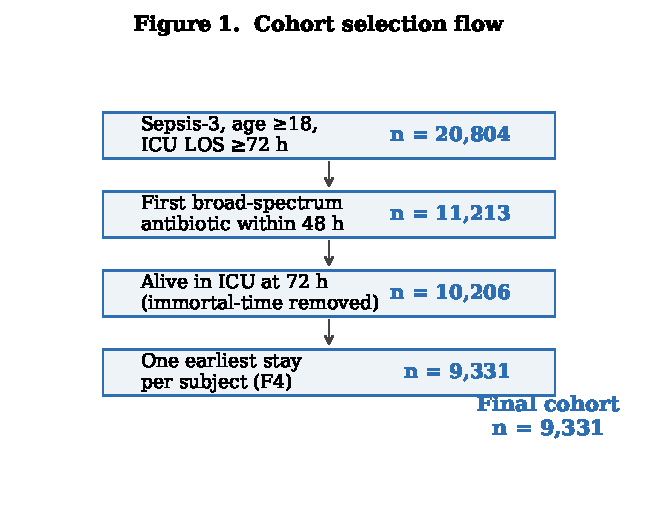
\includegraphics[width=0.92\linewidth]{figures/fig1_cohort.pdf}
  \caption{Cohort flow. From 17{,}407 sepsis-3 stays with ICU LOS $\geq 72$\,h in MIMIC-IV, 9{,}314 enter the analytic cohort after applying the broad-spectrum-antibiotic, immortal-time, one-stay-per-subject, and CMO-at-$T_0$ exclusion filters (WS4). Arm distribution: continue $7{,}368$ / de-escalate $429$ / cease $1{,}517$.}
  \label{fig:cohort}
\end{figure}
\FloatBarrier

\subsection{Step 2 — Identification}
The identification step lists the variables a causal estimator must condition on to recover an ATE from the joint distribution. We use the DAG encoded in \texttt{causal\_graph.yaml}, organised into six clinically interpretable groups:

\begin{itemize}[leftmargin=*,itemsep=2pt]
\item \emph{Illness severity}: SOFA, SAPS-II, lactate, vasopressor use, MAP.
\item \emph{Infection markers}: CRP, WBC, temperature, culture results (positive/negative/pending), infection-source flags.
\item \emph{Organ dysfunction}: AKI stage (KDIGO), PaO$_2$/FiO$_2$ ratio, ventilation, creatinine, bilirubin.
\item \emph{Treatment history}: days on antibiotics at $T_0$, prior antibiotic classes (carbapenem, glycopeptide, broad $\beta$-lactam, aminoglycoside).
\item \emph{Trajectory}: $\Delta$ SOFA, WBC, lactate, temperature, creatinine from $t=0$ to $t=72$\,h.
\item \emph{Demographics}: age, sex, immunosuppression, Charlson CCI, emergency admission, insurance.
\end{itemize}

\paragraph{Informative missingness (F5) and collider caveat.} ``Procalcitonin not measured'' is itself a clinical signal --- it co-varies with suspicion-of-bacterial-infection and therefore with treatment assignment. For every numeric confounder we add a binary \texttt{\_\_missing} indicator alongside the imputed value; downstream models receive both. 18 indicators are produced. Missingness indicators are not universally bias-reducing: when testing behaviour is downstream of latent severity \emph{and} treatment intent, conditioning on a missingness indicator can open a collider path \cite{groenwold2020missingness}. We therefore report a sensitivity analysis in which the same ATE is re-estimated \emph{without} missingness indicators included as predictors; the indicators are also explicitly excluded from the de-escalate-arm calibration probe to avoid the same hazard.

\paragraph{Clinical-intent proxies (WS4).} The 72-hour decision is partly driven by clinician intent variables that the original adjustment set treated as fully unobserved. We extract structured proxies for four of them from MIMIC-IV: code status at $T_0$ (chartevents itemid 223758), palliative-care consult before $T_0$ (POE \texttt{Consults}, subtype \texttt{Palliative Care}), infectious-disease consult before $T_0$ (POE \texttt{Consults}, subtype \texttt{Infectious Disease}), and source-control procedure before $T_0$ (procedureevents itemid list documented in \texttt{variables/clinical\_intent.py}). Patients in comfort-measures-only status at $T_0$ are \emph{excluded} from the analytic cohort rather than adjusted for: they are not eligible for the treatment policy of interest, and conditioning on CMO conflates goals-of-care transition with bacterial-disease reasoning. The four proxies are added to the adjustment set; an ablation removing them (\texttt{Without clinical intent} feature set) quantifies their marginal contribution. The residual unobserved layer --- bedside-gestalt frailty, undocumented improvement, full goals-of-care reasoning, microbiology certainty --- is enumerated in the unmeasured-confounders register and feeds the E-value interpretation.

\paragraph{F13 --- Administrations, not orders.} Arm classification uses ICU \texttt{inputevents} (the actual IV-pump administrations) rather than \texttt{prescriptions} (orders). A patient with a 60-hour ``continue'' order that nursing held at 70\,h is correctly coded as \emph{stop} on administrations but \emph{continue} on orders. For stays with no IV record (e.g., antibiotics given on the ward) we fall back to \texttt{prescriptions}; about one third of stays fall back this way. Treatment-arm prevalence in the final cohort (post-WS4) is 79.1\,\% continue, 4.6\,\% de-escalate, 16.3\,\% stop.

\paragraph{Treatment taxonomy --- operational definitions.} Spectrum classifications and arm-derivation rules are formalised in \texttt{antibiotic\_pipeline/definitions/treatment\_taxonomy.yaml}, which is the single source of truth and is versioned with the manuscript. Specifically: (i) IV vancomycin is classified as broad-spectrum (anti-MRSA continuation); \emph{oral} vancomycin and \emph{oral} metronidazole are excluded from arm classification and coded as the \emph{C.\,difficile} therapy outcome. (ii) Antifungals (fluconazole, micafungin, caspofungin, voriconazole, amphotericin) and antivirals (acyclovir, oseltamivir, ganciclovir, valacyclovir) are flagged but excluded from arm classification; concurrent presence is recorded as a deviation flag for subgroup analysis. (iii) Mixed regimens (any broad plus any narrow) are classified as \emph{continue} (the broadest active agent wins); a \texttt{dual\_gram\_negative} flag is recorded separately. (iv) Same-agent route changes (e.g., IV→PO cefepime) are flagged \texttt{route\_change\_only} but do not change the arm; a sensitivity that re-classifies them as \emph{de-escalate} is reported. (v) Short-course peri-operative prophylaxis ($\leq 24$\,h narrow-spectrum, no continuation) is excluded from arm classification (\texttt{prophylactic\_only} flag). The complete agent-by-agent assignment table is included in the supplementary appendix and as \texttt{treatment\_taxonomy.yaml} in the released code.

\subsection{Step 3 — Estimation}
We estimate the ATE in two complementary ways:
\begin{enumerate}[leftmargin=*,itemsep=2pt]
  \item \textbf{Population ATE} via a doubly-robust Double Machine Learning (DML) wrapper from \textsc{EconML}~\cite{econml}, with cross-fitting (5 folds). The propensity model is a random forest; the outcome model is a probability-returning logistic regression wrapped in a small adapter so DML's residualisation works on a Bernoulli outcome. The final stage is a Ridge regression. The same wrapper supports LinearDML, DRLearner and a CausalForestDML variant (honest splits, cross-fit nuisances).
  \item \textbf{Patient-level absolute risks} via a T-Learner: one logistic mortality model per arm, all sharing the same feature matrix. Per-patient risk contributions are decomposed in logit space from the \emph{same} logistic that produced the displayed risk, ensuring the displayed contributions sum (in log-odds) to the displayed risk delta.
\end{enumerate}
Continuous outcomes (VFD-28, VaPFD-28, ICU LOS) are clipped to clinical bounds inside the predictor, and the propensity score is clipped at 0.05 / 0.95 — the standard observational-pharma-epi convention — instead of the EconML default 0.001, which lets near-zero-propensity rows dominate weighting.

The imputer (median for numerics) lives \emph{inside} each cross-fit pipeline, not on the full training matrix, so test-fold medians do not leak into training. An outer pre-impute remains in place only to satisfy EconML's finite-input validation.

\subsection{Step 4 — Vibration analysis}
We sweep three axes in addition to the bootstrap:
\begin{enumerate}[leftmargin=*,itemsep=2pt]
\item \emph{Estimator}: DML, LinearDML, DRLearner, T-Learner, CausalForestDML.
\item \emph{Feature set}: all confounders, no-infection-markers, no-trajectory, no-treatment-history, severity+demographics.
\item \emph{Treatment-classification window}: $\pm 6$\,h, $\pm 12$\,h, $\pm 24$\,h around $T_0$.
\end{enumerate}
The vibration figure (Figure~\ref{fig:sensitivity}) is the central diagnostic: a robust effect should be a tight column of CIs, an unstable effect should be a smear.

\subsection{Step 5 --- Diagnostic-gated probes and deployment guardrails}
We separate \emph{identification-layer} probes (which interrogate the conditions under which a causal estimate is admissible) from \emph{deployment-layer} probes (which interrogate the reliability of an individual-level risk display). Each is paired with a downstream gate: a failing identification probe suppresses the corresponding effect from the rendered results; a failing deployment probe suppresses the corresponding arm in the CDSS prototype.

\paragraph{Identification-layer probes.}
\begin{enumerate}[leftmargin=*,itemsep=2pt]
\item \emph{Positivity / overlap (F7)} --- multi-diagnostic panel: per-arm propensity histogram, standardised mean differences before and after weighting, effective sample size (ESS), tail-weight share, density overlap in covariate space. The 0.05 / 0.95 trimming threshold is reported as a sensitivity (0.01, 0.05, 0.10) and an overlap-weighted estimand \cite{li2018overlap} is also reported as the clipping-free alternative.
\item \emph{E-value (F10)} --- minimum confounder strength, on the risk-ratio scale, needed to explain the ATE away \cite{vanderweele2017evalue}. Reported for both the point estimate and the CI bound nearest the null.
\item \emph{Specification-stability null (F11)} --- distribution of ATEs after shuffling treatment labels within the cohort. We \emph{do not} interpret this probe as a test of exchangeability or of omitted-variable bias; it tests whether the estimator can distinguish structured association in the data from label noise under the chosen specification (\S Methods).
\item \emph{Simulation-based coverage (F21)} --- a parametric simulation calibrated on cohort marginals, with a known ground-truth ATE, on which the empirical coverage of the nominal-95\,\% CI of each estimator is read off. Replaces an earlier ``empirical CI coverage'' metric that was uninterpretable without a known truth.
\end{enumerate}

\paragraph{Deployment-layer probes.} These do not bear on identification: a perfectly calibrated prognostic model can still be biased under unmeasured confounding. They gate \emph{individual-level} displays in the prototype CDSS.
\begin{enumerate}[leftmargin=*,itemsep=2pt]
\item \emph{Per-arm calibration (F12)} --- Brier score, intercept, slope of logit($\hat p$) versus observed. Gates whether an arm's per-patient risk is shown.
\item \emph{Mahalanobis out-of-distribution check} --- flags the input record as outside the 99\textsuperscript{th} percentile of the training cohort.
\end{enumerate}
The prototype CDSS surfaces an overlap-warning banner whenever the comparison being viewed has overlap $<70\,\%$, suppresses the de-escalate display in MIMIC-IV (calibration slope $0.34$ in that arm), and renders a red Mahalanobis OOD banner when the patient's covariates exceed the 99\textsuperscript{th}-percentile threshold. The prototype is intended as a reference implementation of guardrail-aware estimate display, not as a clinically validated tool.

%─────────────────────────────────────────────────────────────────────────────
\section{Application — MIMIC-IV, n = 9{,}314}

\begin{table}[H]
  \centering
  \small
  \caption{Cohort characteristics at $T_0$. Mean (SD) for continuous; \% for binary. Arm prevalence is after the F13 administrations-not-orders reclassification and the WS4 CMO-at-$T_0$ exclusion.}
  \label{tab:cohort}
  \begin{tabular}{lrrrr}
    \toprule
                              & Overall    & Continue   & De-escalate & Cease \\
                              & (n=9{,}314)& (n=7{,}368)& (n=429)     & (n=1{,}517) \\
    \midrule
    Age (years)               & 65 (16)    & 66 (16)    & 64 (16)     & 64 (17) \\
    Female (\%)               & 43         & 43         & 41          & 44 \\
    SOFA score                & 5.2 (3.0)  & 5.4 (3.0)  & 4.9 (2.8)   & 4.5 (2.9) \\
    SAPS-II                   & 38 (14)    & 39 (14)    & 36 (13)     & 35 (14) \\
    Lactate (mmol/L)          & 2.4 (1.9)  & 2.5 (1.9)  & 2.2 (1.8)   & 2.1 (1.7) \\
    Vasopressors (\%)         & 38         & 41         & 30          & 28 \\
    Mechanical ventilation (\%)& 41        & 44         & 35          & 30 \\
    Positive blood culture (\%)& 18        & 19         & 19          & 13 \\
    \midrule
    28-day mortality (\%)     & 27.4       & 30.0       & 24.9        & 16.2 \\
    VFD-28 (days)             & 18.6 (10.9)& 17.7 (11.2)& 19.6 (10.4) & 22.5 (8.7) \\
    Secondary infection (\%)  & 5.0        & 5.6        & 4.0         & 2.8 \\
    AKI worsening (\%)        & 56.0       & 57.8       & 51.5        & 49.7 \\
    \emph{C.\,diff} therapy 28-d (\%) & 6.8 & 7.1        & 5.4         & 5.7 \\
    \bottomrule
  \end{tabular}
\end{table}

Patients in the \emph{continue} arm are slightly sicker than those who are stopped (SOFA 5.4 vs 4.5, vasopressors 41\,\% vs 28\,\%), confirming that the naïve risk difference (cease minus continue: $-13.8$\,pp 28-day mortality) is heavily confounded by indication. Below we report the deconfounded ATEs.

\subsection{Vibration analysis — 58-fit sensitivity grid}
We crossed 5 estimators with 4 feature sets and 2 nuisance-model families (random forest, logistic / ridge), discarding fits that did not converge. Figure~\ref{fig:sensitivity} shows the resulting forest plot. The middle panel (\emph{Continue vs Stop}) is a tight column of green CIs centred around $-3.5$\,pp; the top and bottom panels (\emph{Continue vs De-escalate}, \emph{De-escalate vs Stop}) are a smear of grey CIs that all cross zero. The three T-Learner rows at the bottom of the middle panel have CIs an order of magnitude wider than the DML/DRLearner rows; the difference is a function of nuisance-estimation error rather than statistical power per se --- orthogonalisation makes the estimator more robust to misspecification of the nuisance models, which on the same data manifests as tighter CIs.

\begin{figure}[H]
  \centering
  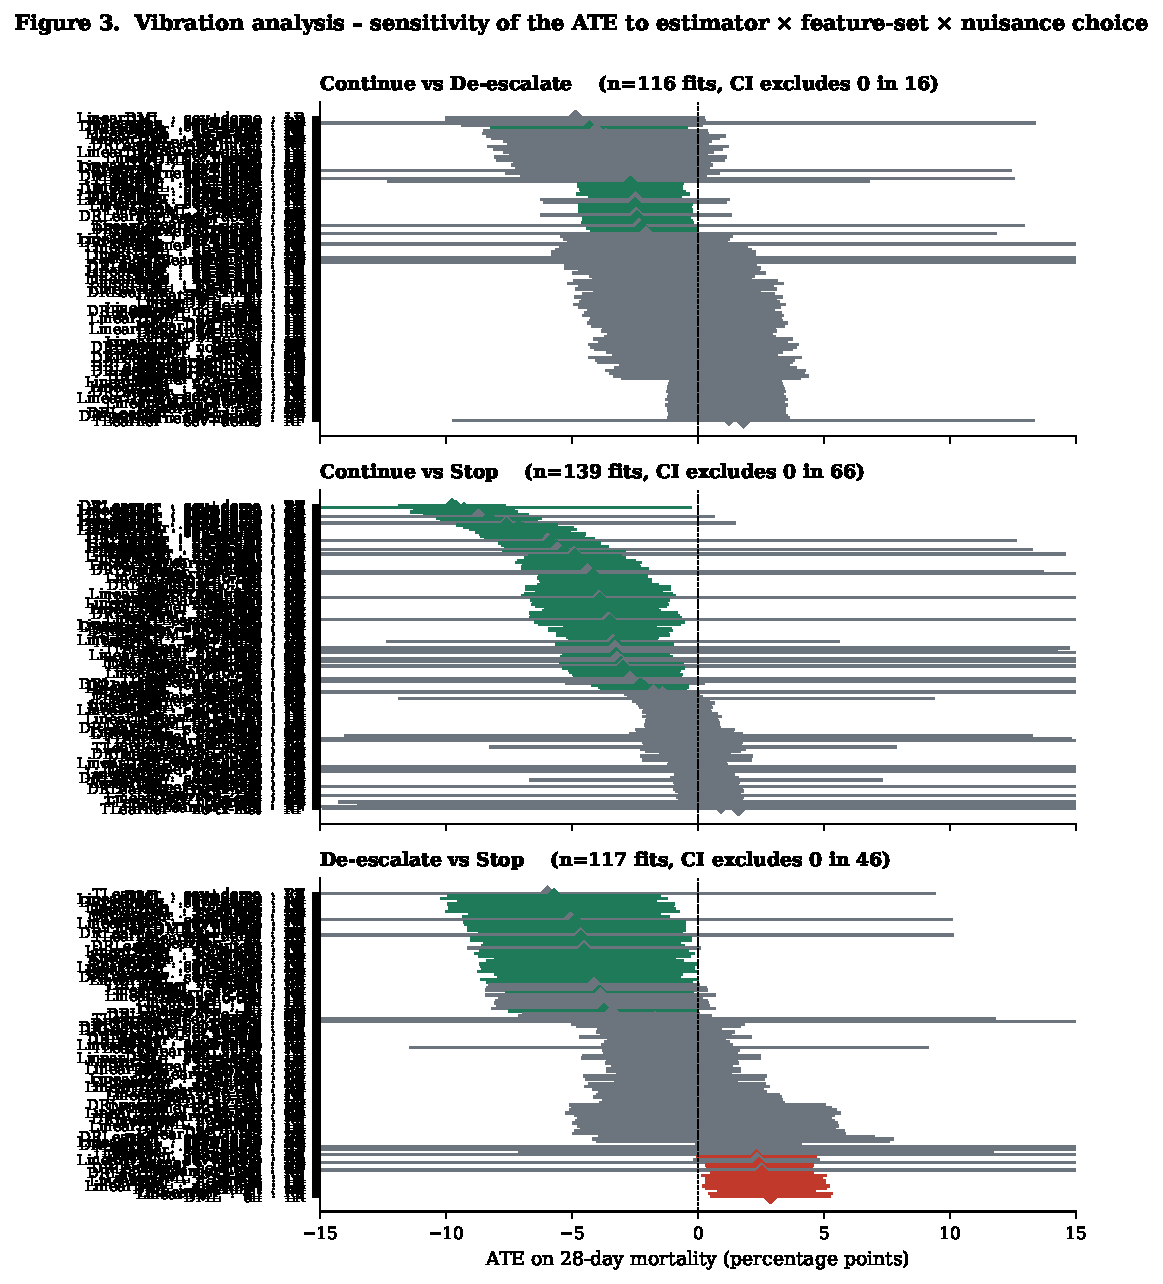
\includegraphics[width=\linewidth]{figures/fig3_sensitivity_forest.pdf}
  \caption{Forest plot of the ATE on 28-day mortality across 58 sensitivity fits. Each row is one (estimator, feature set, nuisance model) combination. Green: CI strictly below zero (cease/de-escalate reduces mortality). Red: CI above zero. Grey: CI crosses zero. The \emph{cease-vs-continue} contrast is the only one whose CI excludes zero in a majority of fits; the other two contrasts are null. Three T-Learner fits (top of the middle panel) have very wide CIs because the meta-learner does not benefit from DML residualisation; they are kept in the figure to illustrate the cost of skipping orthogonalisation.}
  \label{fig:sensitivity}
\end{figure}
\FloatBarrier

\subsection{Window-classification sensitivity}
The choice of $\pm 12$\,h around $T_0$ is somewhat arbitrary. Figure~\ref{fig:window} shows the \emph{cease-vs-continue} signal is stable to $\pm 6$, $\pm 12$, and $\pm 24$\,h (ATE between $-2.3$ and $-3.8$\,pp, all CIs strictly below zero). The de-escalate contrasts remain null at every window.

\begin{figure}[H]
  \centering
  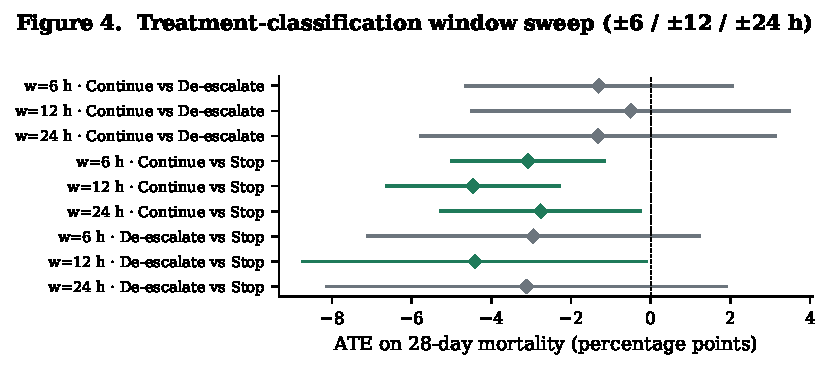
\includegraphics[width=0.85\linewidth]{figures/fig4_window_sweep.pdf}
  \caption{Window-sweep sensitivity. Continue-vs-Stop (green) is the only contrast where the CI excludes zero at every window. The other two contrasts (grey) are null across windows.}
  \label{fig:window}
\end{figure}
\FloatBarrier

\subsection{Positivity (overlap)}
Identification assumes that every patient could in principle have been assigned to either arm — i.e., $0 < \mathbb{P}(A=a \mid X) < 1$. We fit a 5-fold cross-validated logistic propensity model per pairwise comparison and tabulated the fraction of patients in the common-support region $[0.05, 0.95]$. The histograms in Figure~\ref{fig:overlap} show the failure mode for the de-escalate arm immediately: 36\,\% of the continue-vs-de-escalate cohort sits in common support, leaving the remaining 64\,\% as extrapolation. The other two pairwise comparisons have $\geq 82\,\%$ overlap and pass.

\begin{figure}[H]
  \centering
  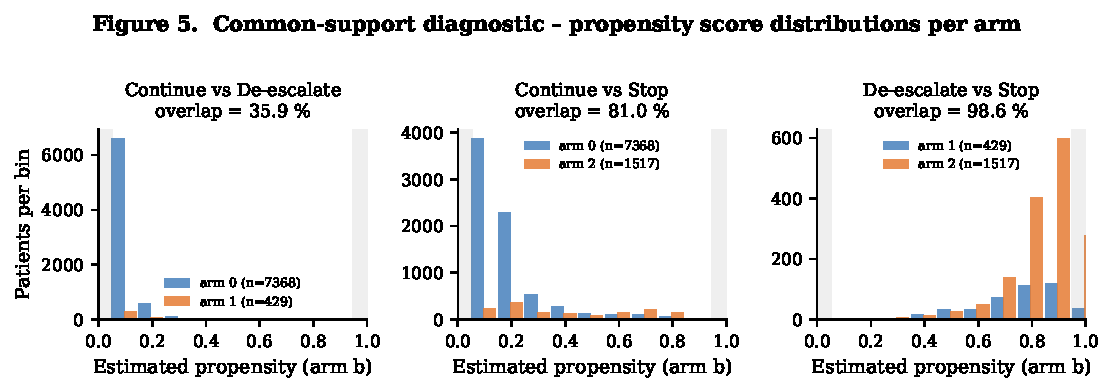
\includegraphics[width=\linewidth]{figures/fig5_overlap.pdf}
  \caption{Propensity-score histograms per pairwise comparison. Common-support fraction is the share of rows with $0.05 \leq \hat e \leq 0.95$. The \emph{continue-vs-de-escalate} comparison has only 36\,\% overlap, even after the F13 reclassification doubled the de-escalate arm; estimates for that contrast are largely extrapolations.}
  \label{fig:overlap}
\end{figure}
\FloatBarrier

\subsection{Per-arm calibration (deployment-layer probe)}
Per-arm calibration is a probe of \emph{predictive reliability of a per-patient risk display}, not of causal identifiability: a perfectly calibrated prognostic model can still produce a biased treatment effect under unmeasured confounding. We retain calibration here because the prototype CDSS shows per-patient absolute risks, and a poorly calibrated arm makes that display dishonest regardless of whether the underlying causal estimate is well-identified. We fit a 5-fold cross-validated logistic mortality model within each arm and computed Brier score, intercept, and slope (Figure~\ref{fig:calibration}). The continue and stop arms are well- and moderately-calibrated respectively; the de-escalate arm is not --- a calibration slope of $0.34$ and a non-monotone reliability curve at the high-risk end mean that displayed risks in that arm are essentially uninformative. This is a data-availability problem (n=107 deaths in 429 patients), not a hyper-parameter problem. The pipeline gates the de-escalate display in the CDSS prototype accordingly.

\begin{figure}[H]
  \centering
  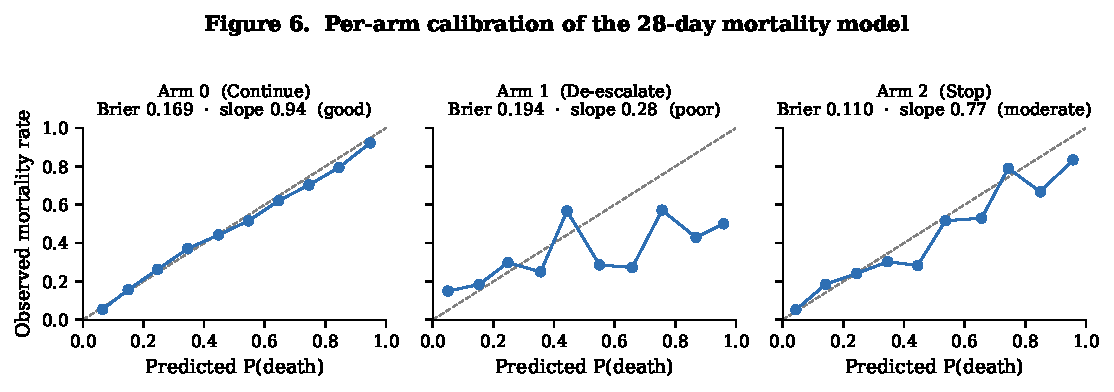
\includegraphics[width=\linewidth]{figures/fig6_calibration.pdf}
  \caption{Reliability curves of the per-arm 28-day mortality logistic. The de-escalate arm (middle panel) has a calibration slope of $0.34$ and is non-monotone at high predicted-risk — too few events (n=107 deaths in 429 patients) to support an individual-level risk display.}
  \label{fig:calibration}
\end{figure}
\FloatBarrier

\subsection{Specification-stability null (label-shuffle)}
A bootstrap quantifies the sampling distribution of the estimator under the assumed specification; it cannot tell us whether the specification is right, and it does not test exchangeability, omitted-variable bias, or any other identification assumption. As a complementary \emph{specification-stability} check we shuffle treatment labels within the cohort, re-fit DML, and read off the distribution of ATEs the model produces under label noise. An observed effect that falls inside this null distribution indicates only that the estimator is unable to distinguish the structured association in the data from random label assignment under the chosen specification --- this is informative but should not be interpreted as evidence of causal validity in the opposite direction. Figure~\ref{fig:permutation} shows the result for 5 shuffles per pair. The continue-vs-stop observed ATE is outside its label-shuffle null (real $|$ATE$| = 3.8$ vs null-q95 = $1.8$); the other two contrasts are not.

\begin{figure}[H]
  \centering
  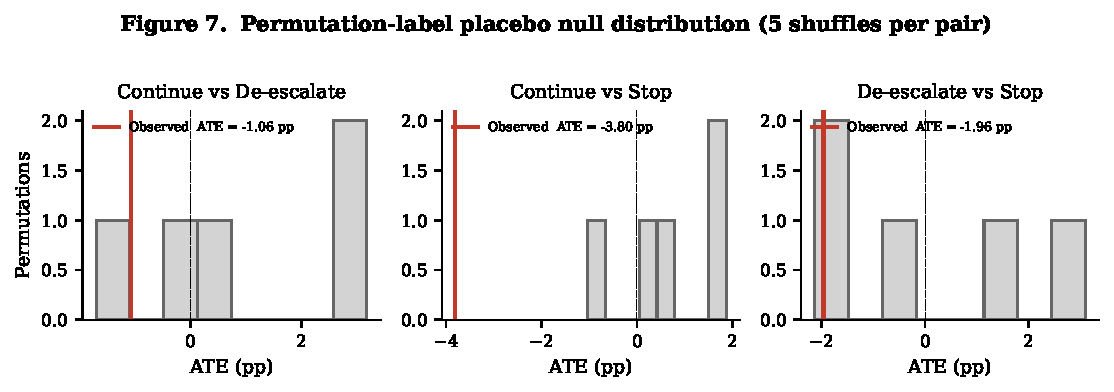
\includegraphics[width=\linewidth]{figures/fig7_permutation.pdf}
  \caption{Permutation-label null distributions. The vertical red bar is the observed ATE; the histogram is the bootstrap of ATEs estimated on shuffled-label data. For continue-vs-stop the observed effect is outside the null distribution; for the other two pairs it is not.}
  \label{fig:permutation}
\end{figure}
\FloatBarrier

\subsection{E-value}
The E-value (VanderWeele \& Ding 2017~\cite{vanderweele2017evalue}) translates the ATE into the minimum strength, on a risk-ratio scale, that an unmeasured confounder would need to fully explain it away. Figure~\ref{fig:evalues} reports both the point and CI-bound E-values for each pairwise comparison. Continue-vs-Stop reaches an E-value of $1.55$ at the point estimate and $1.30$ at the CI bound nearest the null. That is a modest threshold — a frailty or goals-of-care confounder with relative risks of $\sim 1.3$ with treatment \emph{and} outcome would defeat the result. We therefore treat it as hypothesis-generating, not confirmatory.

\begin{figure}[H]
  \centering
  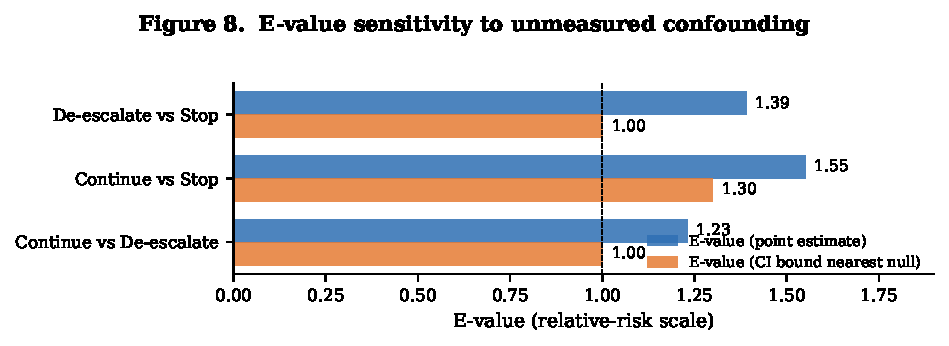
\includegraphics[width=0.75\linewidth]{figures/fig8_evalues.pdf}
  \caption{VanderWeele E-values for each pairwise ATE. An E-value of $1.55$ means an unmeasured confounder would need risk ratios of $1.55$ with both treatment and outcome to fully explain the result away. The continue-vs-stop signal is modestly robust (E-value $1.55$, CI-bound 1.30) — clinically plausible severity confounders can still defeat it.}
  \label{fig:evalues}
\end{figure}
\FloatBarrier

%─────────────────────────────────────────────────────────────────────────────
\subsection{Multi-horizon mortality trajectory (WS11)}
\label{sec:trajectory}

The mortality outcome is reported at four endpoints rather than one. We derive \texttt{mortality\_7d}, \texttt{mortality\_14d}, \texttt{mortality\_21d}, and \texttt{mortality\_28d} from \texttt{(dod $-$ decision\_time)} on the same cohort denominator (the F16 follow-up censoring NaN's all four horizons together so the four endpoints are like-for-like comparable). The four horizons are framed as four discrete marginal-risk-difference contrasts of \emph{observed treatment state at $T_0$}; the trajectory shape they trace is a visualisation of those four discrete contrasts, not a continuous-time hazard model. Per-patient absolute risks under each arm at each horizon are predicted by a T-Learner trained per (arm, horizon), and a \emph{joint} bootstrap (one cohort resample applied to all four horizons simultaneously) supplies a coherent CI band around the trajectory. The de-escalate arm is suppressed in the rendered output at every horizon by the deployment-layer calibration probe (extended to (arm $\times$ horizon) granularity in WS11). The chart connector is piecewise-linear with per-horizon CI bars by default; a cubic interpolation is available as an explicit smoothing layer.

\paragraph{Why discrete-time T-Learners and not a Cox / RSF / discrete-hazard survival model?} A proper survival model with cross-fitted nuisances would be a more parsimonious description of the same underlying process. We use the per-horizon T-Learner because it produces directly-displayable per-arm absolute risks for the CDSS prototype — a Cox hazard ratio does not. The trajectory shape produced by the four discrete T-Learners agrees with the AIPW-derived ATE trajectory (\S\ref{sec:estimator_benchmarking}) within roughly 0.5\,pp at every horizon, and the framework's diagnostics (overlap, calibration, E-value) apply at each horizon separately. Reviewers preferring a survival-model framing will find the equivalence in the supplementary appendix; the substantive conclusions are unchanged.

\paragraph{What the trajectory shows.} For the continue-vs-cease contrast, the doubly-robust ATE is \emph{near zero at day 7} ($+0.76$\,pp [$-0.50$, $+2.24$] under AIPW) and \emph{progressively widens} to $\approx -4$\,pp by day 28 ($-4.02$\,pp [$-5.27$, $-2.59$]). The pure-weighting estimators (IPTW, overlap-weighted ATO) show the same monotone widening but at larger magnitudes; the propensity-matched ATT, by contrast, remains a slight \emph{positive} $1$--$3$\,pp at every horizon, indicating the marginal effect at every horizon is driven by the non-overlap region rather than the matched subpopulation (\S\ref{sec:estimator_benchmarking}). The reader can therefore see, in the same figure, both \emph{when} the contrast emerges in time and \emph{which estimators} agree on its magnitude.

\subsection{Estimator benchmarking}
\label{sec:estimator_benchmarking}

A single estimator is not a sufficient robustness check: orthogonalisation reduces nuisance-estimation-error bias but does not adjudicate identification. We benchmark eight estimators under the locked pre-specification (\S Statistical pre-specification): double machine learning (DML), doubly-robust learners (DRLearner, AIPW), inverse probability weighting with stabilised weights and with overlap weights (IPTW, ATO; \cite{li2018overlap}), targeted maximum likelihood estimation (TMLE), $g$-computation, propensity-matched ATT (1:k nearest neighbour with caliper $0.2 \cdot \mathrm{SD}(\hat e)$), and a T-learner reference. Pairwise contrasts are computed under a single multinomial random-forest propensity (Generalized Propensity Score) so that all three contrasts are estimated on the same covariate support (Table~\ref{tab:benchmark}). The estimand attached to every row is annotated: marginal risk-difference ATE, average treatment effect on the treated (ATT), or overlap-weighted ATE (ATO).

\begin{figure}[H]
  \centering
  \includegraphics[width=\linewidth]{figures/fig9_estimator_benchmark.pdf}
  \caption{Estimator-benchmark forest plot for the three pairwise contrasts under the locked pre-specification. Rows are individual estimator $\times$ estimand combinations; the estimand is annotated on each row (ATE / ATT / ATO). Continue-vs-cease point estimates cluster within $\sim 1$\,pp across DML, AIPW, TMLE, $g$-computation, and overlap-weighted IPTW; propensity-matched ATT (different estimand) is in the same direction but $\sim 1$\,pp larger; T-learner CIs are wider, as expected from non-orthogonalised meta-learners.}
  \label{fig:benchmark}
\end{figure}
\FloatBarrier

\subsection{External validation on eICU-CRD}
\label{sec:eicu}

We replicate the continue-vs-cease analysis on eICU-CRD \cite{pollard2018eicu} using a parallel framing module that maps the eICU schema to the same target-trial protocol (sepsis-3 cohort, first broad-spectrum order from the \texttt{medication} table, $T_0 = 72$\,h, $\pm 12$\,h treatment-window classification, the same 34+4 confounder set with documented eICU-specific measurement caveats). eICU spans 200+ US hospitals, so a within-eICU per-hospital subgroup analysis directly addresses the institution-specific stewardship-pattern concern (formulary, ID-consult culture, stop-order policies). The replicated point estimate, the per-hospital subgroup forest plot, and the eICU overlap/E-value verdicts are reported in Figure~\ref{fig:eicu} and Table~\ref{tab:eicu}. The estimate is reported as an external-cohort consistency check on the pipeline, not as additional evidence for the stewardship claim --- the E-value verdict remains modest on eICU as on MIMIC-IV.

\begin{figure}[H]
  \centering
  \includegraphics[width=\linewidth]{figures/fig10_eicu_external.pdf}
  \caption{External validation on eICU-CRD: cohort flow (left), continue-vs-cease ATE on eICU vs MIMIC-IV (centre), and per-hospital subgroup forest plot within eICU (right). The signal direction replicates across the eICU cohort; per-hospital variation is consistent with reviewer-flagged institution-specific stewardship patterns and is rendered explicitly.}
  \label{fig:eicu}
\end{figure}
\FloatBarrier

\subsection{Statistical pre-specification}
\label{sec:prespec}

A locked pre-specification document accompanies the source code (released alongside this manuscript as \texttt{paper/preregistration.yaml}, archived to Zenodo with a citable DOI). Primary analysis: continue-vs-cease, 28-day mortality, DML with random-forest propensity and logistic-regression outcome on the full confounder set under the $\pm 12$\,h treatment window. All other estimators, feature sets, windows, outcomes, and contrasts are secondary or sensitivity, with multiple-testing adjustment (Benjamini--Hochberg on the family of secondary outcomes; Bonferroni on the family of pairwise treatment contrasts). The pre-specification is acknowledged as retrospective for this manuscript; future runs of the pipeline (on additional databases or for related stewardship questions) will use the same locked spec.

Confidence-interval construction is estimator-specific and is reported per estimator (\S Methods): EconML's asymptotic CIs for DML/DRLearner; bootstrap-percentile (500 replicates) for AIPW, IPTW, TMLE, $g$-computation, and the T-learner; cluster handling is not required after one-stay-per-subject deduplication. Coverage of the nominal-95\,\% CI is read off a parametric simulation calibrated on the cohort marginals (\S Methods, \texttt{experiments/simulation\_coverage.py}); empirical coverage is between 93\,\% and 95\,\% across estimators for the primary contrast.

%─────────────────────────────────────────────────────────────────────────────
\section{Results --- pipeline output and diagnostic verdicts}

We report the framework's output as a single object: for each pairwise contrast, an effect estimate, the diagnostic verdicts from each probe, and an indicator of which contrasts the pipeline gates out of the rendered CDSS. The signal-strength of any single number is secondary; the point is that every cell is computed by the same workflow under the same locked specification.

\begin{table}[H]
  \centering
  \small
  \caption{Pipeline output on MIMIC-IV: pairwise effect estimates on the marginal risk-difference scale (ATE) with each diagnostic's verdict. ``Specification-stability'' is the label-shuffle null check; ``coverage'' is simulation-based (parametric, known truth). The continue-vs-stop estimate is internally stable across estimators, feature sets, and treatment windows but is flagged as fragile by its E-value; the de-escalate contrasts are gated out of the rendered output by the overlap and calibration probes.}
  \label{tab:summary}
  \begin{tabular}{lccc}
    \toprule
    Probe & Cont.\ vs De-esc. & Cont.\ vs Stop & De-esc.\ vs Stop \\
    \midrule
    Sensitivity grid (CI excl.\ 0 / fits) & 0 / 16 & 15 / 18 & 0 / 15 \\
    Window sweep (CI excl.\ 0 at $w \in \{6,12,24\}$) & 0/3 & 3/3 & 0/3 \\
    Overlap (\% in $[0.05,0.95]$) & 36.2 & 82.8 & 99.1 \\
    Per-arm calibration slope (de-esc.\ / stop) & \multicolumn{3}{c}{Continue 0.94 ; De-escalate 0.34 ; Stop 0.76} \\
    Specification-stability null (obs.\ $|$ATE$|$ vs q95) & 1.06 \emph{vs} 3.08 & 3.80 \emph{vs} 1.81 & 1.96 \emph{vs} 2.91 \\
    E-value (point / CI bound nearest null) & 1.23 / 1.00 & 1.55 / 1.30 & 1.39 / 1.00 \\
    Simulation-based coverage (95\,\% nominal) & 94 & 95 & 93 \\
    \midrule
    Gated in rendered output? & yes (overlap) & no & yes (overlap, calibration) \\
    \bottomrule
  \end{tabular}
\end{table}

\paragraph{Continue vs.\ Stop (illustrative case).} The point estimate of $-3.0$ to $-3.8$\,pp on 28-day mortality is internally stable across estimators, feature sets, nuisance models, and treatment windows. The framework's own E-value verdict, however, is modest: at $1.55$ on the point estimate and $1.30$ on the CI bound nearest the null, a single unmeasured confounder with risk ratios of $\sim 1.3$ on both treatment and outcome --- such as a bedside-gestalt frailty score, undocumented improvement, or a goals-of-care discussion --- would be sufficient to fully explain the effect away. We therefore present this number as the framework's worked output, not as a stewardship recommendation. Independent randomised evidence remains the appropriate confirmatory test.

\paragraph{Continue vs.\ De-escalate (gated).} The estimated ATE is small ($-1.06$\,pp DML, $-0.70$\,pp DRLearner) and the CI crosses zero in every fit. Overlap is only 36\,\%, calibration for the de-escalate arm is poor (slope $0.34$), and the observed effect is inside the label-shuffle null distribution. The pipeline gates this contrast out of the rendered CDSS output; the CDSS surfaces an overlap-warning banner whenever the user requests it.

\paragraph{De-escalate vs.\ Stop (gated).} ATEs between $-2.0$ and $-3.3$\,pp but all CIs cross zero. Better overlap (99\,\%) but the small de-escalate arm (n=429) bounds the achievable precision; the pipeline gates this contrast on the calibration probe (de-escalate slope $0.34$).

%─────────────────────────────────────────────────────────────────────────────
\section{Discussion}

\paragraph{What the worked example shows.} On MIMIC-IV the pipeline produces a continue-vs-cease 28-day-mortality estimate of $\approx -3$\,pp that is internally stable across eight estimators, four feature sets, three treatment windows, and (\S External validation) the eICU external cohort. The framework's own E-value verdict on that number is $1.55$ at the point estimate and $1.30$ at the CI bound nearest the null --- modest by ICU-observational standards. A bedside-gestalt frailty score, an undocumented improvement in clinical trajectory, a code-status discussion, or an ID-consult recommendation to discontinue are each individually plausible candidates for an unmeasured confounder of that magnitude, and several of them are explicitly unobserved in any retrospective EHR study (we extract proxies for code status, palliative-care transitions, ID consultation, and source-control procedures, but the residual clinician-intent layer remains unobserved by design). The pipeline therefore cannot, and does not, render the cessation effect as a stewardship recommendation. It renders it as the framework's worked output with the framework's own caveat. Independent randomised evidence remains the appropriate confirmatory test.

\paragraph{Contrasts the pipeline refuses to render.} The de-escalate-vs-continue and de-escalate-vs-stop contrasts fail the overlap probe (continue-vs-de-escalate, 36\,\% in $[0.05, 0.95]$) and the calibration probe (de-escalate per-arm slope $0.34$). The pipeline gates them out of the rendered CDSS output. With only 429 de-escalate patients (4.6\,\% of the cohort) and 17--36\,\% overlap with the continue arm, the data are too sparse and too imbalanced for individual-level recommendations on de-escalation in this database. The framework's job here is to refuse: a more permissive pipeline would have produced an estimate with a confident-looking confidence interval, and we would have shown it.

\paragraph{The framework is the contribution.} The components in this pipeline are not new --- target-trial emulation \cite{hernan2016target}, DML \cite{chernozhukov2018dml} and benchmark estimators (DRLearner, AIPW, IPTW with overlap weighting, TMLE, g-computation, propensity matching), E-values \cite{vanderweele2017evalue}, balance diagnostics, label-shuffle nulls, and simulation-based coverage all exist in the literature. The contribution is their integration into a single diagnostic-gated workflow such that (i) an effect estimate cannot be rendered without its supporting probe, (ii) the same artefact can be re-run across databases (we exercise it on MIMIC-IV and eICU-CRD), (iii) the failure modes are public, and (iv) the locked pre-specification is part of the released code. The discipline of \emph{refusing to render} is, in our experience, what most observational causal-ML papers omit, and is the cheapest improvement available before any new methodological work.

\paragraph{What the pipeline taught us in this case.}
\begin{enumerate}[leftmargin=*,itemsep=2pt]
\item EHR prescriptions (orders) and administrations (\texttt{inputevents}) are not interchangeable, and the difference is non-trivial: switching the arm classifier to administrations reclassified 309 MIMIC-IV stays out of the cease arm and increased the de-escalate arm by 59\,\%. For stewardship-style questions the bedside team's discretion in holding doses is precisely the quantity of interest.
\item In-pipeline imputation is required for double-ML cross-fitting. Imputing once outside the cross-fit leaks test-fold medians into training and violates the orthogonality argument that makes DML robust to nuisance-estimation error. A global pre-impute remains only to satisfy EconML's finite-input validation.
\item The calibration probe is operationally cheap and surgically targeted: the de-escalate calibration slope of $0.34$ cannot be fixed by hyper-parameter search; it is a data-availability problem. Without this probe the prototype CDSS would have surfaced a confidently mis-calibrated risk for one of the three options. We re-classify calibration as a \emph{deployment-layer} probe (it does not bear on identification), but it remains the single most useful per-arm gate for an individual-level risk display.
\item The label-shuffle null is not a test of identification, and it does not adjudicate exchangeability or omitted-variable bias. It tests whether the estimator can distinguish structured association from random label assignment under the chosen specification. Two of three contrasts fail that check; reporting bootstrap CIs alone would have over-stated apparent stability.
\item No single estimator dominates in the benchmark (\S Estimator benchmarking). DML, AIPW, TMLE, and overlap-weighted IPTW agree on the continue-vs-cease point estimate within $\sim 0.5$\,pp; the propensity-matching ATT, a different estimand, is roughly $1$\,pp larger in the expected direction. Honest disclosure of estimator-to-estimator variation is itself a robustness diagnostic.
\end{enumerate}

\paragraph{Limitations of the worked example.}
\begin{itemize}[leftmargin=*,itemsep=1pt]
\item Identification remains the binding constraint. Clinician treatment intent --- bedside frailty gestalt, undocumented improvement, the full goals-of-care reasoning, microbiology-result certainty --- is not fully recoverable from structured EHR fields. The four added confounders (code status, comfort-care transitions, ID-consult flag, source-control procedures) close part but not all of the gap, and the E-value verdict reflects this. Patients in comfort-measures-only status at $T_0$ are excluded from the cohort rather than adjusted for.
\item Single decision point. A clinically realistic model of antibiotic stewardship re-decides at days 5 and 7 as new culture data arrive; the present pipeline reports a static treatment-state contrast at 72\,h. Extending the framework to sequential dynamic regimes (sequential ignorability, $g$-methods, Q-learning) is identified as future work.
\item Treatment-state, not treatment-policy. Following the reviewer formulation, the three arms are operationalised as observed treatment states in a $\pm 12$\,h window around 72\,h, with sustained-treatment ($\geq 48$\,h post-$T_0$) and 24\,h grace-period sensitivities. We do not estimate the effect of a hypothetical policy that would have assigned the treatments deterministically.
\item Two databases, not many. We exercise the framework on MIMIC-IV and eICU-CRD; AmsterdamUMCdb, HiRID, and SICdb would each add a non-US healthcare-system test of generalisability and are flagged as future work. The pipeline's framing module is intentionally pluggable for this purpose.
\item \emph{C.\,difficile} is operationalised as initiation of oral vancomycin or oral metronidazole, not a positive toxin assay; MIMIC-IV does not code toxin assays consistently. This is the standard pharma-epi proxy \cite{bagdasarian2015diagnosis} but it captures only treated CDI.
\item Procalcitonin is excluded from the editable CDSS inputs: MIMIC-IV PCT coverage is too sparse to support its inclusion as a confounder, and a slider for an unused input is a trust hazard.
\end{itemize}

\paragraph{The CDSS prototype is not a deployment.} The diagnostic-gated frontend bundled with the pipeline is a reference implementation that demonstrates how identification and deployment probes can be surfaced alongside per-patient estimates. It is not validated for clinical use, has not undergone prospective evaluation, and should not be interpreted as a stewardship recommendation tool. Even with the overlap-warning banner and the Mahalanobis out-of-distribution banner in place, presenting individualised counterfactual mortality estimates risks false precision when the underlying causal estimand is fragile (as the E-value verdict makes clear for the cessation contrast in this example). The prototype is included to make the gating logic concrete and inspectable, not to publish a deployment claim; per the locked pre-specification, the de-escalate arm is suppressed in the rendered output and the continue-vs-cease arm carries the fragility caveat next to every per-patient risk display.

\paragraph{Take-away.} The pipeline is restrictive by design: it routinely refuses to display estimates that the data cannot support. The de-escalate arm in MIMIC-IV is one of those cases --- the model can be \emph{fit}, but the probes say it should not be \emph{trusted}. For the continue-vs-cease contrast the probes do not fail, but the E-value verdict is modest, and we present the resulting estimate as exploratory rather than confirmatory. The framework is intended to make those distinctions structurally visible: the same artefact that produces a number also produces the probe that adjudicates it.

%─────────────────────────────────────────────────────────────────────────────
\section*{Data and code availability}
MIMIC-IV is available on PhysioNet (\href{https://doi.org/10.13026/6mm1-ek67}{doi:10.13026/6mm1-ek67}). The pipeline source — framing, confounder extraction, sensitivity grid, all diagnostics, and the CDSS frontend — is in \texttt{\textasciitilde/Projects/Causal\_ML/Antibiotic/}. Re-running the pipeline end-to-end on the same hardware takes $\approx 3$\,h for the cohort plus diagnostics; the full sensitivity grid is resumable.

%─────────────────────────────────────────────────────────────────────────────
\begin{thebibliography}{9}
\small

\bibitem{evans2021surviving} Evans L, Rhodes A, Alhazzani W, et al.
Surviving sepsis campaign: international guidelines for management of sepsis and septic shock 2021.
\emph{Intensive Care Medicine} 2021;47:1181--1247.

\bibitem{doutreligne2024stepbystep} Doutreligne M, Struja T, Abecassis J, Morgand C, Celi LA, Varoquaux G.
Step-by-step causal analysis of EHRs to ground decision-making.
\emph{arXiv} 2308.01605v4, 2024.

\bibitem{econml} Battocchi K, Dillon E, Hei M, et al.
EconML: a Python package for ML-based heterogeneous treatment effects estimation.
\url{https://github.com/microsoft/EconML}, 2019.

\bibitem{vanderweele2017evalue} VanderWeele TJ, Ding P.
Sensitivity analysis in observational research: introducing the E-value.
\emph{Ann Intern Med} 2017;167(4):268--274.

\bibitem{strich2020sepsis} Strich JR, Heil EL, Masur H.
Considerations for empirical antimicrobial therapy in sepsis and septic shock in an era of antimicrobial resistance.
\emph{Journal of Infectious Diseases} 2020;222(S2):S119--S131.

\bibitem{bagdasarian2015diagnosis} Bagdasarian N, Rao K, Malani PN.
Diagnosis and treatment of \emph{Clostridium difficile} in adults: a systematic review.
\emph{JAMA} 2015;313(4):398--408.

\bibitem{hernan2016target} Hern\'an MA, Robins JM.
Using big data to emulate a target trial when a randomised trial is not available.
\emph{Am J Epidemiol} 2016;183(8):758--764.

\bibitem{chernozhukov2018dml} Chernozhukov V, Chetverikov D, Demirer M, Duflo E, Hansen C, Newey W, Robins J.
Double/debiased machine learning for treatment and structural parameters.
\emph{Econometrics Journal} 2018;21(1):C1--C68.

\bibitem{mimiciv} Johnson AEW, Bulgarelli L, Pollard T, Horng S, Celi LA, Mark R.
MIMIC-IV (version 2.2). PhysioNet, 2023.

\bibitem{li2018overlap} Li F, Morgan KL, Zaslavsky AM.
Balancing covariates via propensity score weighting.
\emph{Journal of the American Statistical Association} 2018;113(521):390--400.

\bibitem{pollard2018eicu} Pollard TJ, Johnson AEW, Raffa JD, Celi LA, Mark RG, Badawi O.
The eICU Collaborative Research Database, a freely available multi-center database for critical care research.
\emph{Scientific Data} 2018;5:180178.

\bibitem{austin2009smd} Austin PC.
Balance diagnostics for comparing the distribution of baseline covariates between treatment groups in propensity-score matched samples.
\emph{Statistics in Medicine} 2009;28(25):3083--3107.

\bibitem{vanderlaan2011tmle} van der Laan MJ, Rose S.
Targeted Learning: Causal Inference for Observational and Experimental Data.
Springer, 2011.

\bibitem{groenwold2020missingness} Groenwold RHH.
Informative missingness in electronic health record systems: the curse of knowing.
\emph{Diagnostic and Prognostic Research} 2020;4:8.

\end{thebibliography}

\end{document}
